%\documentclass[a4paper]{article}

\usepackage[spanish, es-tabla, es-noshorthands]{babel}
\usepackage[table,xcdraw]{xcolor}
\usepackage[a4paper, footnotesep=1.25cm, headheight=1.25cm, top=2.54cm, left=2.54cm, bottom=2.54cm, right=2.54cm]{geometry}
%\geometry{showframe}

%\usepackage{wrapfig}			%Wrap figure in text
\usepackage[export]{adjustbox}	%Move images
\usepackage{changepage}			%Move tables

\usepackage{tikz}
\usepackage{amsmath}
\usepackage{amsfonts}
\usepackage{amssymb}
\usepackage{float}
\usepackage{graphicx}

\usepackage{caption}
\usepackage{subcaption}
\usepackage{multicol}
\usepackage{multirow}
\usepackage{wrapfig}
\setlength{\doublerulesep}{\arrayrulewidth}
\usepackage{booktabs}
\usepackage[numbib, nottoc, notlot, notlof]{tocbibind}

\usepackage{hyperref}
\hypersetup{
    colorlinks=true,
    linkcolor=blue,
    filecolor=magenta,      
    urlcolor=blue,
    citecolor=blue,    
}

%Change Font Size

% #1 = size, #2 = text
\newcommand{\setparagraphsize}[2]{{\fontsize{#1}{6}\selectfont#2 \par}}		%Cambia el size de todo el parrafo
\newcommand{\setlinesize}[2]{{\fontsize{#1}{6}\selectfont#2}}				%Cambia el font de una oración

\newcommand{\note}[1]{
	\begin{center}
		\huge{ \textcolor{red}{#1} }
	\end{center}
}

%FONTS (IMPORTANTE): Compilar en XeLaTex o LuaLaTeX
\usepackage{anyfontsize}	%Font size
\usepackage{fontspec}		%Font type

\usepackage{etoolbox}
\usepackage{todonotes}

\newcommand{\observacion}[2]{  \ifnumequal{1}{#1}{ { \todo[inline,backgroundcolor=red!25,bordercolor=red!100]{\textbf{Observación: #2}} } }{  }  }

\setcounter{topnumber}{2}
\setcounter{bottomnumber}{2}
\setcounter{totalnumber}{4}
\renewcommand{\topfraction}{0.85}
\renewcommand{\bottomfraction}{0.85}
\renewcommand{\textfraction}{0.15}
\renewcommand{\floatpagefraction}{0.8}
\renewcommand{\textfraction}{0.1}
\setlength{\floatsep}{5pt plus 2pt minus 2pt}
\setlength{\textfloatsep}{5pt plus 2pt minus 2pt}
\setlength{\intextsep}{5pt plus 2pt minus 2pt}

\newcommand{\quotes}[1]{``#1''}
\usepackage{array}
\newcolumntype{C}[1]{>{\centering\let\newline\\\arraybackslash\hspace{0pt}}m{#1}}
\usepackage[american]{circuitikz}
\usetikzlibrary{calc}
\usepackage{fancyhdr}
\usepackage{units} 



\pagestyle{fancy}
\fancyhf{}
\lhead{IA.03 - Inteligencia Artificial}
\rhead{Lambertucci, Mestanza}
\rfoot{Página \thepage}

\usepackage{listings}

\usepackage{color} %red, green, blue, yellow, cyan, magenta, black, white
\definecolor{mygreen}{RGB}{28,172,0} % color values Red, Green, Blue
\definecolor{mylilas}{RGB}{170,55,241}
%Items con bullets y no cuadrados
\renewcommand{\labelitemi}{\textbullet }
\lstset{language=R,%
    %basicstyle=\color{red},
    breaklines=true,%
    morekeywords={matlab2tikz},
    keywordstyle=\color{blue},%
    morekeywords=[2]{1}, keywordstyle=[2]{\color{black}},
    identifierstyle=\color{black},%
    stringstyle=\color{mylilas},
    commentstyle=\color{mygreen},%
    showstringspaces=false,%without this there will be a symbol in the places where there is a space
    numbers=left,%
    numberstyle={\tiny \color{black}},% size of the numbers
    numbersep=9pt, % this defines how far the numbers are from the text
    emph=[1]{for,end,break},emphstyle=[1]\color{red}, %some words to emphasise
    %emph=[2]{word1,word2}, emphstyle=[2]{style},    
    literate=
    	{á}{{\'a}}1 {é}{{\'e}}1 {í}{{\'i}}1 {ó}{{\'o}}1 {ú}{{\'u}}1
  		{Á}{{\'A}}1 {É}{{\'E}}1 {Í}{{\'I}}1 {Ó}{{\'O}}1 {Ú}{{\'U}}1
		{à}{{\`a}}1 {è}{{\`e}}1 {ì}{{\`i}}1 {ò}{{\`o}}1 {ù}{{\`u}}1
  		{À}{{\`A}}1 {È}{{\'E}}1 {Ì}{{\`I}}1 {Ò}{{\`O}}1 {Ù}{{\`U}}1
  		{ä}{{\"a}}1 {ë}{{\"e}}1 {ï}{{\"i}}1 {ö}{{\"o}}1 {ü}{{\"u}}1
  		{Ä}{{\"A}}1 {Ë}{{\"E}}1 {Ï}{{\"I}}1 {Ö}{{\"O}}1 {Ü}{{\"U}}1
  		{â}{{\^a}}1 {ê}{{\^e}}1 {î}{{\^i}}1 {ô}{{\^o}}1 {û}{{\^u}}1
  		{Â}{{\^A}}1 {Ê}{{\^E}}1 {Î}{{\^I}}1 {Ô}{{\^O}}1 {Û}{{\^U}}1
  		{Ã}{{\~A}}1 {ã}{{\~a}}1 {Õ}{{\~O}}1 {õ}{{\~o}}1
  		{œ}{{\oe}}1 {Œ}{{\OE}}1 {æ}{{\ae}}1 {Æ}{{\AE}}1 {ß}{{\ss}}1
  		{ű}{{\H{u}}}1 {Ű}{{\H{U}}}1 {ő}{{\H{o}}}1 {Ő}{{\H{O}}}1
  		{ç}{{\c c}}1 {Ç}{{\c C}}1 {ø}{{\o}}1 {å}{{\r a}}1 {Å}{{\r A}}1
  		{€}{{\euro}}1 {£}{{\pounds}}1 {«}{{\guillemotleft}}1
  		{»}{{\guillemotright}}1 {ñ}{{\~n}}1 {Ñ}{{\~N}}1 {¿}{{?`}}1,
  	inputencoding=latin1,
}

%\begin{document}
%
\subsection{Consigna}

\section*{Parte A – Análisis Exploratorio de Datos}

\begin{enumerate}
    \item Abra en R la base Glass de la librería mlbench.
    \begin{verbatim}
    library(mlbench)
    data(Glass)
    \end{verbatim}
    Muestre \texttt{dim(Glass)}. ¿Cuántos ejemplos de vidrio tiene la base?
    
    \item Escriba en R \texttt{?Glass} y copie aquí la Descripción (\textit{Description}) que aparece en la página web.
    
    \item Abra la página web de Glass en UCI (Universidad de California) \url{https://archive.ics.uci.edu/ml/datasets/glass+identification}. Busque la sección “Additional Variable Information” y luego \textit{Class Labels}. Copie aquí los tipos de vidrio de la base. ¿Cuál tipo de vidrio no está representado en la base (none in this database)?
    
    \item La variable a predecir es \texttt{Type} que representa los tipos de vidrios. Muestre un \textit{summary} de la base \texttt{summary(Glass)}.
    
    \item Indique cuántos vidrios hay de cada clase. \texttt{summary(Glass\$Type)}
    
    \item A grandes rasgos, los tipos de vidrio serían (hay 2 tipos de ventana de edificio):
    \begin{itemize}
        \item Ventana de edificio
        \item Ventana de automóvil
        \item Recipiente
        \item Vajilla
        \item Faro de Auto
    \end{itemize}
    Busque y muestre una imagen de cada tipo de vidrio. Indique para cada
    imagen la página web origen de la misma.
    
    \item Renombre cada categoría y transforme la variable \texttt{Type} a factor. Luego renombre \texttt{Type} como \texttt{TipoDeVidrio}.
    \begin{verbatim}
    Glass$Type=as.character(Glass$Type)
    Glass$Type[Glass$Type=="1"]="VentanaTipo1"
    Glass$Type[Glass$Type=="2"]="VentanaEdificio"
    Glass$Type[Glass$Type=="3"]="VentanaAuto"
    Glass$Type[Glass$Type=="5"]="Recipiente"
    Glass$Type[Glass$Type=="6"]="Vajilla"
    Glass$Type[Glass$Type=="7"]="FaroAuto"
    Glass$Type=factor(Glass$Type)
    names(Glass)[names(Glass)=="Type"]="TipoDeVidrio"
    \end{verbatim}
    Muestre un \texttt{summary(Glass)} para ver cómo quedó.
    
    \item Realice un gráfico de barras de la variable \texttt{Glass\$TipoDeVidrio}. Amplíe el gráfico para ver los nombres de los tipos de vidrio.
    \begin{verbatim}
    plot(Glass$TipoDeVidrio, main="Gráfico de barras de Título", col="COLOR")
    \end{verbatim}
    \begin{itemize}
        \item[a)] Para el título ingrese su nombre, como “Gráfico de barras de Marcela”.
        \item[b)] Elija un color para el gráfico. Tenga en cuenta que si ingresa \texttt{colors()} en R, verá que hay más de 500 colores posibles.
        \item[c)] Indique el código R utilizado.
    \end{itemize}
\end{enumerate}

\section*{Parte B – Conjuntos}

\begin{enumerate}
    \setcounter{enumi}{1}
    \item Muestre un \texttt{head} y un \texttt{summary} del conjunto de entrenamiento y del conjunto de testeo.
    \begin{verbatim}
    head(entreno)
    summary(entreno)
    head(testeo)
    summary(testeo)
    \end{verbatim}
    
    \item ¿Cuántos registros quedaron en cada conjunto (entrenamiento y testeo) en total?
    \begin{verbatim}
    dim(Glass)
    dim(entreno)
    dim(testeo)
    \end{verbatim}
    
    \item ¿Cuántos registros de cada número quedaron en cada conjunto?
    \begin{verbatim}
    table(Glass$TipoDeVidrio)
    table(entreno$TipoDeVidrio)
    table(testeo$TipoDeVidrio)
    \end{verbatim}
\end{enumerate}

\section*{Parte C – Árbol de Decisión}

\begin{enumerate}
    \item Cargue la librería \texttt{rpart} y cree un Árbol de Decisión para modelar el problema planteado.
    \begin{verbatim}
    arbol=rpart(TipoDeVidrio~., entreno, method="class")
    \end{verbatim}
    Cargue la librería \texttt{rpart.plot} y grafique el Árbol de Decisión resultante (utilice el parámetro \texttt{cex=0.8} para una mejor visualización).
    \begin{verbatim}
    rpart.plot(arbol, extra=1, type=5, cex=0.8)
    \end{verbatim}
    
    \item ¿Cuántas hojas tiene el Árbol de Decisión?
    
    \item Según el Árbol de Decisión creado, ¿cuándo un vidrio es del tipo “FaroAuto”? (Indique las reglas siguiendo las ramas desde el nodo raíz hasta las hojas “FaroAuto”.)
    
    \item Calcule la matriz de confusión utilizando la instrucción \texttt{confusionMatrix} de la librería \texttt{caret}. Muestre una captura de pantalla de los resultados completos (la matriz de confusión, \textit{accuracy} y tablas).
    \begin{verbatim}
    pred=predict(arbol, testeo, type="class")
    confusionMatrix(pred, testeo$TipoDeVidrio)
    \end{verbatim}
    
    \item La cantidad de elementos de la matriz de confusión es igual a la cantidad de elementos de testeo (o sea \texttt{dim(testeo)}) Sume la cantidad de elementos de la diagonal de la matriz de confusión y divida el resultado por dim(testeo).
Muestre la cuenta con números y muestre que es igual al accuracy.
\item Vea la tabla Statistics by Class debajo de la matriz de confusión e indique cuál clase presenta menor sensibilidad.
\item Con la instrucción Glass[numVidrio,] podemos obtener los datos de un vidrio de la base base[filas,columnas]Considere los 2 últimos números de su DNI (2numDNI) y busque el vidrio de esa fila
vidrioAsignado=Glass[2numDNI,] vidrioAsignado
Transcriba los datos del vidrio de ese número. ¿Qué tipo de vidrio es?
\item Prediga con el Árbol de Decisión el vidrio de los 2 últimos números de su DNI predict(arbol,vidrioAsignado,type="class")
¿Coincide la predicción con lo esperado?
\end{enumerate}

\section*{Parte D – Optimización del modelo}

\begin{enumerate}
    \item Creación de un Árbol de Decisión sin algunas restricciones
    
    Con la instrucción \texttt{arbol\$control} se pueden ver las restricciones en la creación del Árbol de Decisión. Cree un Árbol de Decisión sin algunas de las restricciones con la siguiente instrucción:
    
    \begin{verbatim}
    arbolGrande=rpart(TipoDeVidrio~., entreno, method="class", cp=0, minsplit=0)
    \end{verbatim}
    
    \item Dibujar el Árbol de Decisión
    
    Dibuje el Árbol de Decisión utilizando la siguiente instrucción:
    
    \begin{verbatim}
    rpart.plot(arbolGrande, extra=1, type=5, cex=0.6)
    \end{verbatim}
    
    \item Mostrar el gráfico plotcp
    
    Muestre el gráfico \texttt{plotcp(arbolGrande)}. Amplíe el gráfico para ver más cps.
    
    Cada parte de este gráfico es la siguiente:
    
    \begin{itemize}
        \item En la parte inferior del gráfico figura el cp (parámetro de complejidad) de cada Árbol de Decisión.
        \item En la parte superior la cantidad de hojas.
        \item En el eje vertical el error de cada modelo (calculado por cross validation).
        \begin{figure}[H]
	\centering
	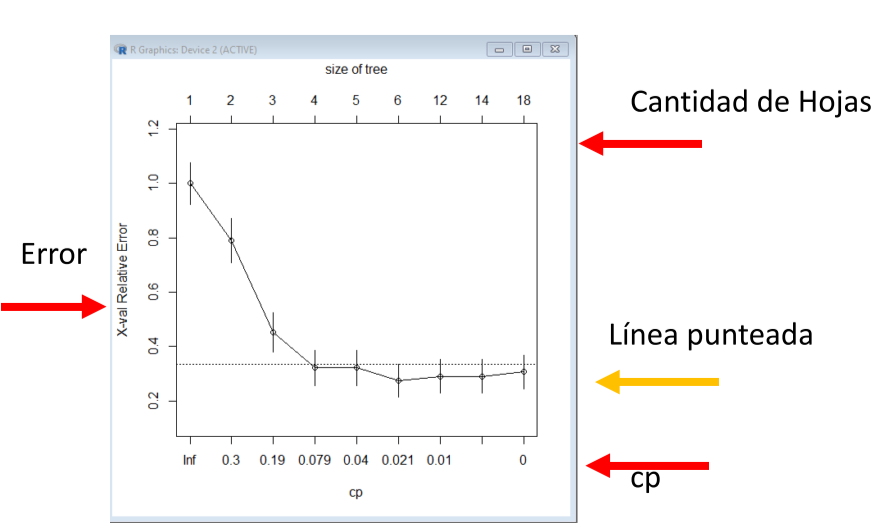
\includegraphics[width=\linewidth]{../Ejercicio-2/ImagenesEjercicio2/consigna.png}
	\end{figure}
    \end{itemize}
\end{enumerate}
\begin{enumerate}
    \setcounter{enumi}{3}
    \item Elija un \texttt{cp} del gráfico, cuyo error (eje vertical) esté por debajo de la línea punteada (el \texttt{cp} elegido debe figurar en el gráfico).
    \begin{verbatim}
    arbolPodado=prune(arbolGrande, cp=cpElegido)
    \end{verbatim}
    Indique el código R utilizado.
    
    \item Muestre una captura de pantalla de los resultados completos (la matriz de confusión, \textit{accuracy} y tablas) del Árbol de Decisión podado. ¿Mejoró el modelo?
    \begin{verbatim}
    pred=predict(arbolPodado, testeo, type="class")
    confusionMatrix(pred, testeo$TipoDeVidrio)
    \end{verbatim}
    Verifique \textit{accuracy}, y sensibilidades y especificidades de cada categoría. Tal vez el \textit{accuracy} no mejoró, pero alguna categoría mejoró la sensibilidad.
\end{enumerate}

\section*{Parte E – Parte Teórica}

Resuma en un párrafo lo realizado en este TP.

\subsection{Análisis Exploratorio de Datos}
\subsubsection{Desarrollo}
Lo primero que se hace es el análisis exploratorio de datos, se comienza por leer la descripción del dataset a utilizar, la cual es:
"A data frame with 214 observation containing examples of the chemical analysis of 7 different types of glass. The problem is to forecast the type of class on basis of the chemical analysis. The study of classification of types of glass was motivated by criminological investigation. At the scene of the crime, the glass left can be used as evidence (if it is correctly identified!)."\\
A continuación se obtiene la cantidad de observaciones y variables con las que se cuenta, son 214 muestras y 10 variables. Este dataset trata acerca de vidrios, en particular se busca predecir el tipo de vidrio en función de la composición quimica de los mismos. Los tipos de vidrio son:
\begin{table}[H]
\centering
\begin{tabular}{|c|c|}
\hline
\textbf{Valor} & \textbf{Descripción}                                                                                       \\ \hline
1              & building\_windows\_float\_processed                                                                        \\ \hline
2              & building\_windows\_non\_float\_processed                                                                   \\ \hline
3              & vehicle\_windows\_float\_processed                                                                         \\ \hline
4              & \begin{tabular}[c]{@{}c@{}}vehicle\_windows\_non\_float\_processed \\ (none in this database)\end{tabular} \\ \hline
5              & containers                                                                                                 \\ \hline
6              & tableware                                                                                                  \\ \hline
7              & headlamps                                                                                                  \\ \hline
\end{tabular}
\caption{Tipos de vidrios.}
\label{tab:classLabels}
\end{table}
Cabe mencionar que hay un vidrio que no está representado, este es el 4 (la ventana del vehículo que no está procesada).
Continuando con el análisis exploratorio de datos se procede a ver un summary de la base.
\begin{table}[h]
    \centering
    \begin{tabular}{|c|c|c|c|c|c|c|c|c|}
    \hline
    RI & Na & Mg & Al & Si & K & Ca & Ba & Fe \\ \hline
    Min. & 1.511 & 10.73 & 0.000 & 0.290 & 69.81 & 0.000 & 5.430 & 0.000 \\ \hline
    1st Qu. & 1.517 & 12.91 & 2.115 & 1.190 & 72.28 & 0.000 & 8.240 & 0.000 \\ \hline
    Median & 1.518 & 13.30 & 3.480 & 1.360 & 72.79 & 0.000 & 8.600 & 0.000 \\ \hline
    Mean & 1.518 & 13.41 & 2.685 & 1.445 & 72.65 & 0.175 & 8.957 & 0.057 \\ \hline
    3rd Qu. & 1.519 & 13.82 & 3.600 & 1.630 & 73.09 & 0.000 & 9.172 & 0.100 \\ \hline
    Max. & 1.534 & 17.38 & 4.490 & 3.500 & 75.41 & 3.150 & 16.190 & 0.510 \\ \hline
    \end{tabular}
    \caption{Resumen de la base de datos Glass, variables cuantitativas.}
\end{table}

\begin{table}[H]
    \centering
    \begin{tabular}{|c|c|}
    \hline
    Type & Cantidad \\ \hline
    1 & 70 \\
    2 & 76 \\
    3 & 17 \\
    5 & 13 \\
    6 & 9 \\
    7 & 29 \\ \hline
    \end{tabular}
    \caption{Resumen de la base de datos Glass, variables cualitativas.}
     \label{tabCualitativa}
\end{table}
Utilizando las tablas ({\ref{tabCualitativa}}) y ({\ref{tab:classLabels}}) se puede interpretar cuantos vidrios hay de cada tipo.
A manera ilustrativa se procede a mostrar un ejemplo de cada vidrio, ignorando los repetidos (Edificio y faros de auto).

\begin{figure}[H]
    \centering
    \begin{minipage}[b]{0.4\textwidth}
        \centering
        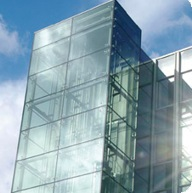
\includegraphics[width=\linewidth]{../Ejercicio-2/ImagenesEjercicio2/buildingGlass.jpg}
        \caption{\href{https://www.doubleglazedwindows.net.au/Acoustic-Windows-and-Doors-Float-Glass.html}{Ventana de edificio}}	
        \label{fig:pic1}
    \end{minipage}
    \hfill
    \begin{minipage}[b]{0.4\textwidth}
        \centering
        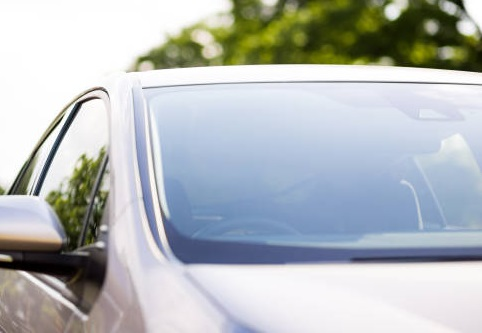
\includegraphics[width=\linewidth]{../Ejercicio-2/ImagenesEjercicio2/carwindowGlass.jpg}
        \caption{\href{https://www.valleyglass.com/custom-vehicles/}{Ventana de automóvil}}	
        \label{fig:pic2}
    \end{minipage}
\end{figure}
\begin{figure}[htbp]
    \centering
    \begin{minipage}[b]{0.4\textwidth}
        \centering
        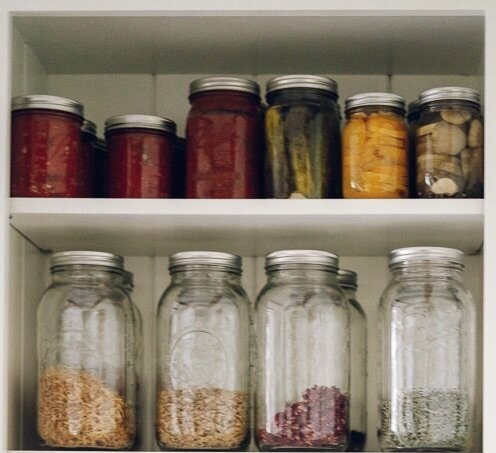
\includegraphics[width=\linewidth]{../Ejercicio-2/ImagenesEjercicio2/containerGlass.jpg}
        \caption{\href{https://thewellco.co/glass-food-storage-jars}{Recipiente}}	
        \label{fig:pic3}
    \end{minipage}
    \hfill
    \begin{minipage}[b]{0.4\textwidth}
        \centering
        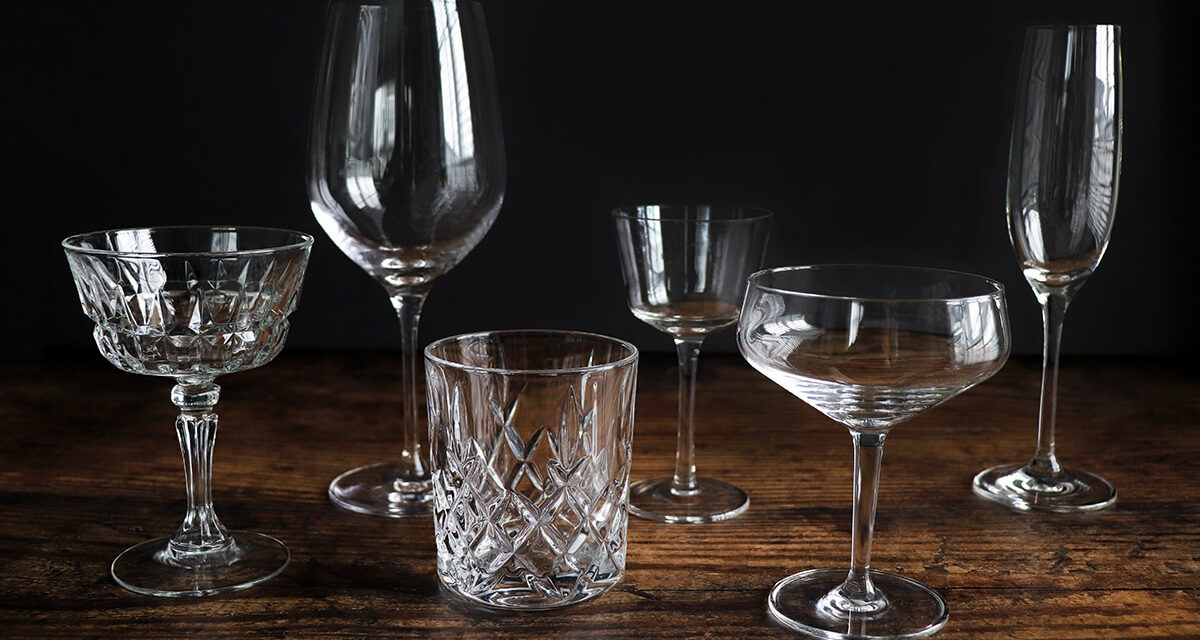
\includegraphics[width=\linewidth]{../Ejercicio-2/ImagenesEjercicio2/tablewareGlass.jpg}
        \caption{\href{https://casualmixologist.com/guides/mixology-basics/glassware-explained}{Vajilla}}	
        \label{fig:pic4}
    \end{minipage}
\end{figure}
\begin{figure}[H]
	\centering
	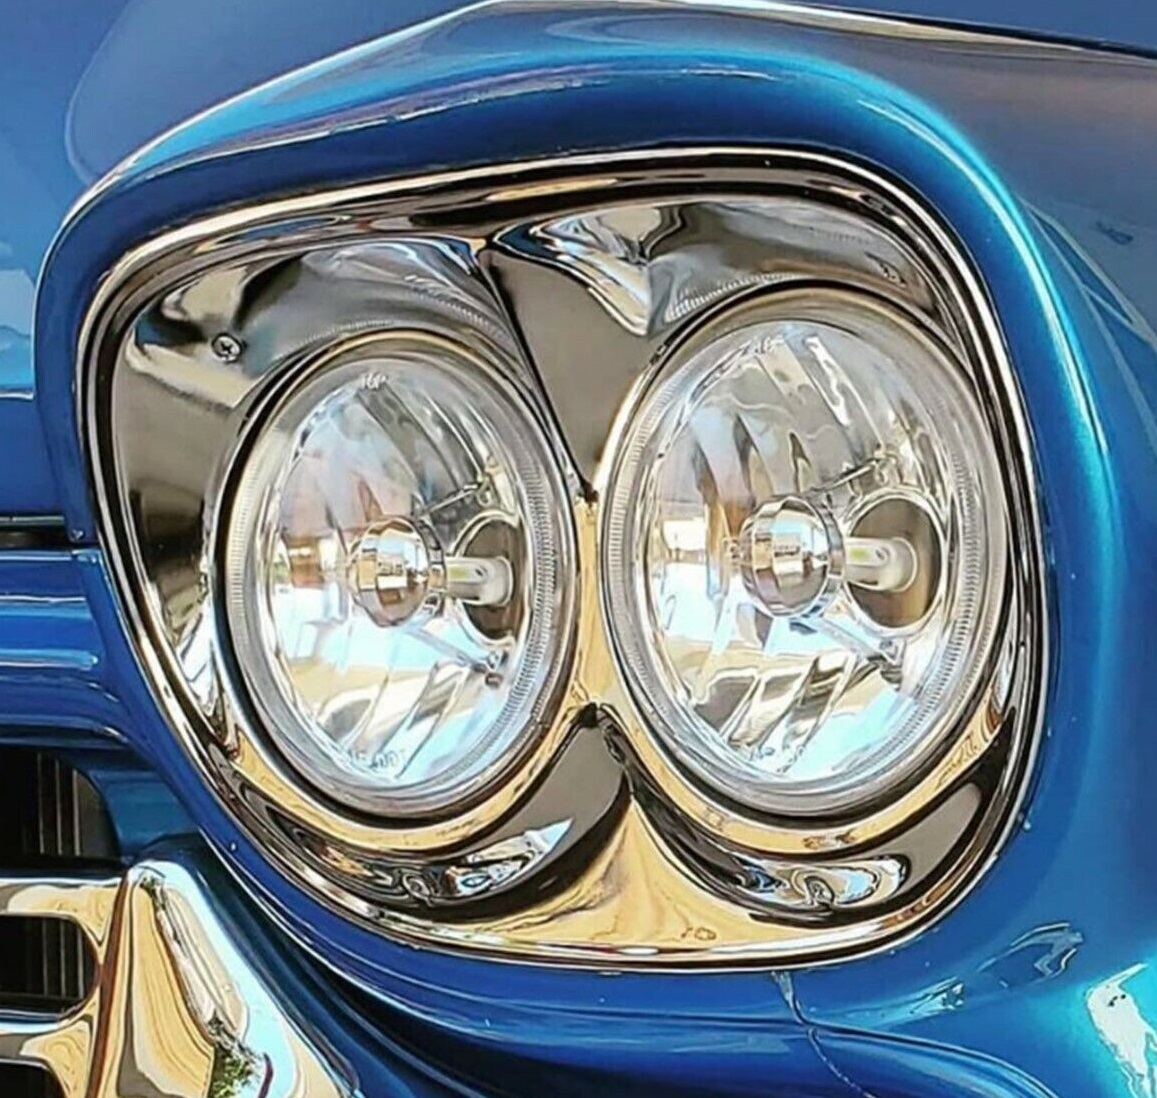
\includegraphics[width=.5\linewidth]{../Ejercicio-2/ImagenesEjercicio2/headlightGlass.jpg}
	\caption{\href{https://www.octanelighting.com/5-34-crystal-clear-metal-glass-headlight-led-set-033-034-g5-led-2.html}{Faro de auto}}	
	\label{fig:pic5}
\end{figure}
Luego se renombró la variable 'type' a 'TipoDeVidrio' y se asigno por cada numero una etiqueta en particular.

\begin{table}[H]
\centering
\begin{tabular}{|c|c|}
\hline
\textbf{Valor previo} & \textbf{Descripción} \\ \hline
1                     & VentanaTipo1         \\ \hline
2                     & VentanaEdificio      \\ \hline
3                     & VentanaAuto          \\ \hline
5                     & Recipiente           \\ \hline
6                     & Vajilla              \\ \hline
7                     & FaroAuto             \\ \hline
\end{tabular}

\caption{Tabla de variables.}
\label{tab:newnames}
\end{table}


Finalmente se grafica un histograma de la variable TipoDeVidrio.

\begin{figure}[H]
	\centering
	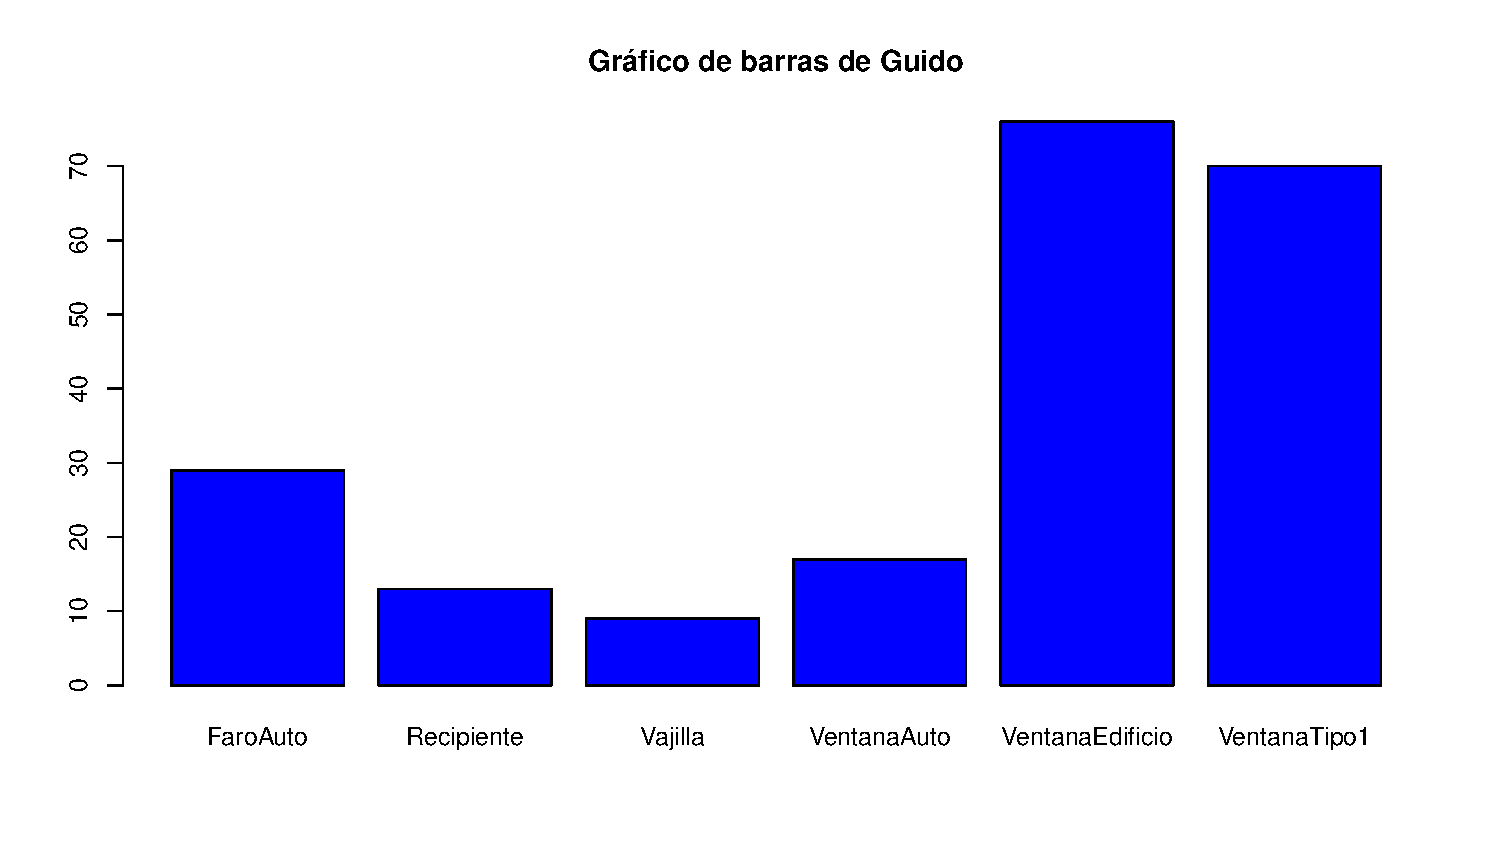
\includegraphics[width=\linewidth]{../Ejercicio-2/ImagenesEjercicio2/TipoDeVidrio.pdf}
	\caption{Histograma de la variable "TipoDeVidrio".}	
	\label{fig:tipodevdrio}
\end{figure}
\subsubsection{Código utilizado}
\lstinputlisting[language=R]{../../../Code/Ej1b/EDA.R}
\subsection{Conjuntos}
Lo siguiente es separar en dos conjuntos el dataset, siendo estos el conjunto de entrenamiento y testeo. Esto es fundamental para corroborar que el modelo efectivamente logro generalizar información y no "aprenderse" el dataset (Overfitting).
La semilla utilizada es 40397224, y la proporción de particion es p=0.75.
\lstinputlisting[language=R]{../../../Code/Ej1b/asd.R}
Luego de generar la partición se hace un head() y un summary() de estos.
Al hacer un head() a entreno queda:

\begin{table}[H]
    \centering
    \begin{tabular}{ccccccccccl}
        \toprule
        RI & Na & Mg & Al & Si & K & Ca & Ba & Fe & TipoDeVidrio \\
        \midrule
        1.52101 & 13.64 & 4.49 & 1.10 & 71.78 & 0.06 & 8.75 & 0 & 0.00 & VentanaTipo1 \\
        1.51761 & 13.89 & 3.60 & 1.36 & 72.73 & 0.48 & 7.83 & 0 & 0.00 & VentanaTipo1 \\
        1.51742 & 13.27 & 3.62 & 1.24 & 73.08 & 0.55 & 8.07 & 0 & 0.00 & VentanaTipo1 \\
        1.51596 & 12.79 & 3.61 & 1.62 & 72.97 & 0.64 & 8.07 & 0 & 0.26 & VentanaTipo1 \\
        1.51756 & 13.15 & 3.61 & 1.05 & 73.24 & 0.57 & 8.24 & 0 & 0.00 & VentanaTipo1 \\
        1.51755 & 13.00 & 3.60 & 1.36 & 72.99 & 0.57 & 8.40 & 0 & 0.11 & VentanaTipo1 \\
        \bottomrule
    \end{tabular}
    \caption{Head de entreno}
    \label{tab:vidrio}
\end{table}
Si se hace un summary() :
\begin{table}[H]
  \centering
  \begin{tabular}{ccccccccccl}
    \toprule
    & RI & Na & Mg & Al & Si & K & Ca & Ba & Fe & TipoDeVidrio \\
    \midrule
    Min.    & 1.511 & 10.73 & 0.000 & 0.340 & 69.81 & 0.0000 & 5.430 & 0.000 & 0.00000 & FaroAuto:22 \\
    1st Qu. & 1.517 & 12.91 & 2.277 & 1.202 & 72.23 & 0.1225 & 8.225 & 0.000 & 0.00000 & Recipiente:10 \\
    Median  & 1.518 & 13.30 & 3.480 & 1.410 & 72.77 & 0.5500 & 8.565 & 0.000 & 0.00000 & Vajilla:7 \\
    Mean    & 1.518 & 13.44 & 2.760 & 1.467 & 72.61 & 0.5165 & 8.823 & 0.197 & 0.05173 & VentanaAuto:13 \\
    3rd Qu. & 1.519 & 13.82 & 3.610 & 1.667 & 73.10 & 0.6100 & 9.070 & 0.000 & 0.07750 & VentanaEdificio:57 \\
    Max.    & 1.531 & 17.38 & 4.490 & 3.500 & 75.41 & 6.2100 & 14.680 & 3.150 & 0.51000 & VentanaTipo1:53 \\
    \bottomrule
  \end{tabular}
  \caption{Summary de entreno}
  \label{tabla_descripcion}

\end{table}

Y lo mismo correspondiente a testeo:
\begin{table}[H]
  \centering
  \begin{tabular}{ccccccccccl}
    \toprule
    RI & Na & Mg & Al & Si & K & Ca & Ba & Fe & TipoDeVidrio \\
    \midrule
    3 & 1.51618 & 13.53 & 3.55 & 1.54 & 72.99 & 0.39 & 7.78 & 0 & VentanaTipo1 \\
    4 & 1.51766 & 13.21 & 3.69 & 1.29 & 72.61 & 0.57 & 8.22 & 0 & VentanaTipo1 \\
    7 & 1.51743 & 13.30 & 3.60 & 1.14 & 73.09 & 0.58 & 8.17 & 0 & VentanaTipo1 \\
    9 & 1.51918 & 14.04 & 3.58 & 1.37 & 72.08 & 0.56 & 8.30 & 0 & VentanaTipo1 \\
    18 & 1.52196 & 14.36 & 3.85 & 0.89 & 71.36 & 0.15 & 9.15 & 0 & VentanaTipo1 \\
    22 & 1.51966 & 14.77 & 3.75 & 0.29 & 72.02 & 0.03 & 9.00 & 0 & VentanaTipo1 \\
    \bottomrule
  \end{tabular}
  \caption{Head de testeo}
  \label{tabla_ejemplo}
\end{table}
\begin{table}[H]
  \centering

  \begin{tabular}{ccccccccccl}
    \toprule
    & RI & Na & Mg & Al & Si & K & Ca & Ba & Fe & TipoDeVidrio \\
    \midrule
    Min.    & 1.512 & 11.02 & 0.000 & 0.290 & 70.16 & 0.0000 & 7.780 & 0.0000 & 0.00000 & FaroAuto:7 \\
    1st Qu. & 1.517 & 12.92 & 0.000 & 1.117 & 72.36 & 0.1350 & 8.293 & 0.0000 & 0.00000 & Recipiente:3 \\
    Median  & 1.518 & 13.27 & 3.490 & 1.300 & 72.86 & 0.5600 & 8.800 & 0.0000 & 0.00000 & Vajilla:2 \\
    Mean    & 1.519 & 13.31 & 2.449 & 1.376 & 72.77 & 0.4365 & 9.373 & 0.1067 & 0.07346 & VentanaAuto:4 \\
    3rd Qu. & 1.519 & 13.81 & 3.580 & 1.545 & 73.07 & 0.6100 & 9.783 & 0.0000 & 0.14000 & VentanaEdificio:19 \\
    Max.    & 1.534 & 14.94 & 3.850 & 2.790 & 75.18 & 2.7000 & 16.190 & 1.5700 & 0.34000 & VentanaTipo1:17 \\
    \bottomrule
  \end{tabular}
    \caption{Summary de testeo}
  \label{tabla_descripcion}
\end{table}
Las dimensiones finales son (\textasciitilde75$\%$ entreno y \textasciitilde25$\%$ testeo):

\begin{table}[H]
  \centering

  \begin{tabular}{lccccccc}
    \toprule
    & FaroAuto & Recipiente & Vajilla & VentanaAuto & VentanaEdificio & VentanaTipo1 & Total\\
    \midrule
    Glass & 29 & 13 & 9 & 17 & 76 & 70 & 214\\
    entreno & 22 & 10 & 7 & 13 & 57 & 53 & 162\\
    testeo & 7 & 3 & 2 & 4 & 19 & 17 & 52\\
    \bottomrule
  \end{tabular}
    \caption{Descripción de la tabla}
  \label{tabla_ejemplo}
\end{table}



\subsection{Árbol de Decisión}
Utilizando la librería rpart se arma un arbol de decisión. 
\begin{figure}[H]
	\centering
	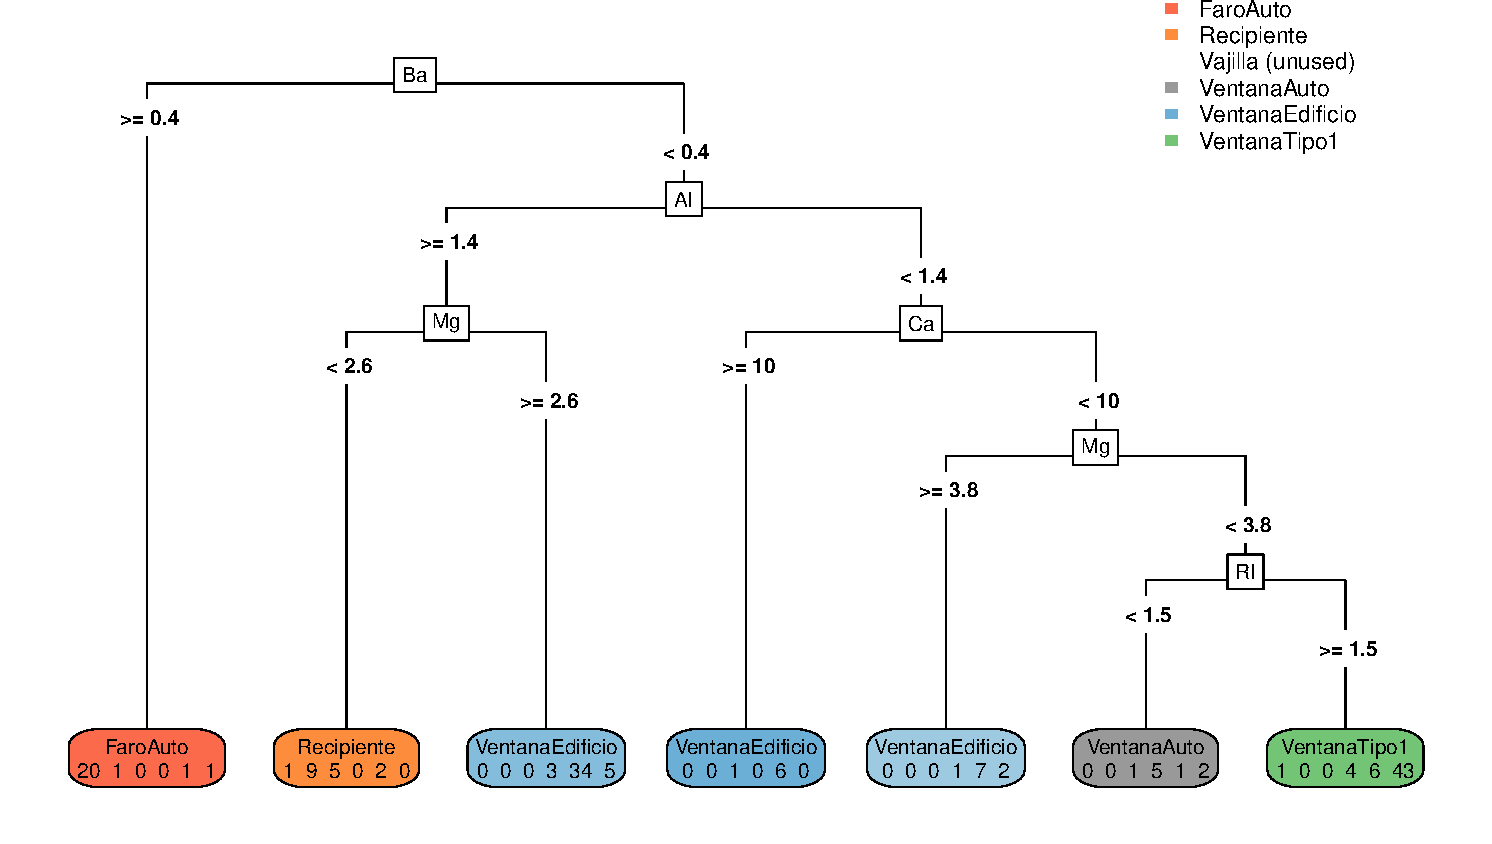
\includegraphics[width=\linewidth]{../Ejercicio-2/ImagenesEjercicio2/add.pdf}
	\caption{Primer árbol de decisión}	
	\label{fig:add11}
\end{figure}
Cuenta con 7 hojas. Para que el árbol decida que una muestra es un faro de auto basta con que el contenido de Bario sea mayor igual a 0.4. A continuación se calcula la matriz de confusión.


\begin{table}[htbp]
  \centering

    \begin{tabular}{l|ccccc}
    \multicolumn{1}{c}{} & \multicolumn{5}{c}{Reference} \\
    \cline{2-6}
    \multirow{6}[2]{*}{\rotatebox[origin=c]{90}{Prediction}} & FaroAuto & Recipiente & Vajilla & VentanaAuto & VentanaEdificio \\
    \cline{2-6}
          & 6     & 0     & 0     & 0     & 0 \\
          & 0     & 2     & 1     & 0     & 2 \\
          & 0     & 0     & 0     & 0     & 0 \\
          & 1     & 0     & 0     & 1     & 3 \\
          & 0     & 1     & 0     & 1     & 10 \\
          & 0     & 0     & 1     & 2     & 4 \\
    \end{tabular}%
      \caption{Matriz de confusión}
  \label{tab:confusion_matrixx}%
\end{table}%

\begin{table}[htbp]
  \centering
    \begin{tabular}{ll}
    \hline
    \textbf{Accuracy} & 0.6346 \\
    \textbf{95\% CI} & (0.4896, 0.7638) \\
    \textbf{No Information Rate} & 0.3654 \\
    \textbf{P-Value [Acc > NIR]} & 7.296e-05 \\
    \textbf{Kappa} & 0.506 \\
    \textbf{Mcnemar's Test P-Value} & NA \\
    \hline
    \end{tabular}%
      \caption{Estadísticas generales}

  \label{tab:overall_stats}%
\end{table}%

\begin{table}[htbp]
  \centering
    \begin{tabular}{lcccccc}
    \hline
          & \textbf{Sensitivity} & \textbf{Specificity} & \textbf{Pos Pred Value} & \textbf{Neg Pred Value} & \textbf{Prevalence} & \textbf{Detection Rate} \\
    \hline
    \textbf{Class: FaroAuto} & 0.8571 & 1.0000 & 1.0000 & 0.9783 & 0.1346 & 0.1154 \\
    \textbf{Class: Recipiente} & 0.66667 & 0.93878 & 0.40000 & 0.97872 & 0.05769 & 0.03846 \\
    \textbf{Class: Vajilla} & 0.00000 & 1.00000 & NaN   & 0.96154 & 0.03846 & 0.00000 \\
    \textbf{Class: VentanaAuto} & 0.25000 & 0.89583 & 0.16667 & 0.93478 & 0.07692 & 0.01923 \\
    \textbf{Class: VentanaEdificio} & 0.5263 & 0.8788 & 0.7143 & 0.7632 & 0.3654 & 0.1923 \\
    \textbf{Class: VentanaTipo1} & 0.8235 & 0.8000 & 0.6667 & 0.9032 & 0.3269 & 0.2692 \\
    \hline
    \end{tabular}%
      \caption{Estadísticas por clase}
  \label{tab:class_stats}%
\end{table}%
Cabe notar que la cantidad de elementos de la matriz de confusión es igual a la cantidad de elementos de testeo. Además se procede a calcular la accuracy utilizando la matriz (\ref{tab:confusion_matrixx}).
\begin{equation}
\text{Accuracy}=\frac{\sum TP+TN}{\sum TP+TN+FP+FN}=\frac{6+2+0+1+10+14}{52} \ = \frac{33}{52} \ \approx \ 0.6346  
\end{equation}
Donde TP es True positive, TN True negative, FP False positive y FN Flase negative. Cabe mencionar que el valor calculado coincide con obtenido por R.
Por otro lado se observa que la categoría con menor sensibilidad corresponde a "Vajilla".\\
Se elije el vidrio en la posicion 24 como muestra, el cual es tipo 'VentanaTipo1'.
\begin{table}[h]
\centering
\begin{tabular}{|c|c|c|c|c|c|c|c|c|c|}
\hline
\textbf{RI} & \textbf{Na} & \textbf{Mg} & \textbf{Al} & \textbf{Si} & \textbf{K} & \textbf{Ca} & \textbf{Ba} & \textbf{Fe} & \textbf{TipoDeVidrio} \\
\hline
1.51 & 12.81 & 3.57 & 1.35 & 73.02 & 0.62 & 8.59 & 0 & 0 & VentanaTipo1 \\
\hline
\end{tabular}
\end{table}
Se prueba el modelo con este vidrio en particular y efectivamente lo predice de manera correcta.

\subsection{Optimización del modelo}
Se crea un árbol de decisión pero obligando a que llegue a la maxima longitud posible.
\begin{figure}[H]
	\centering
	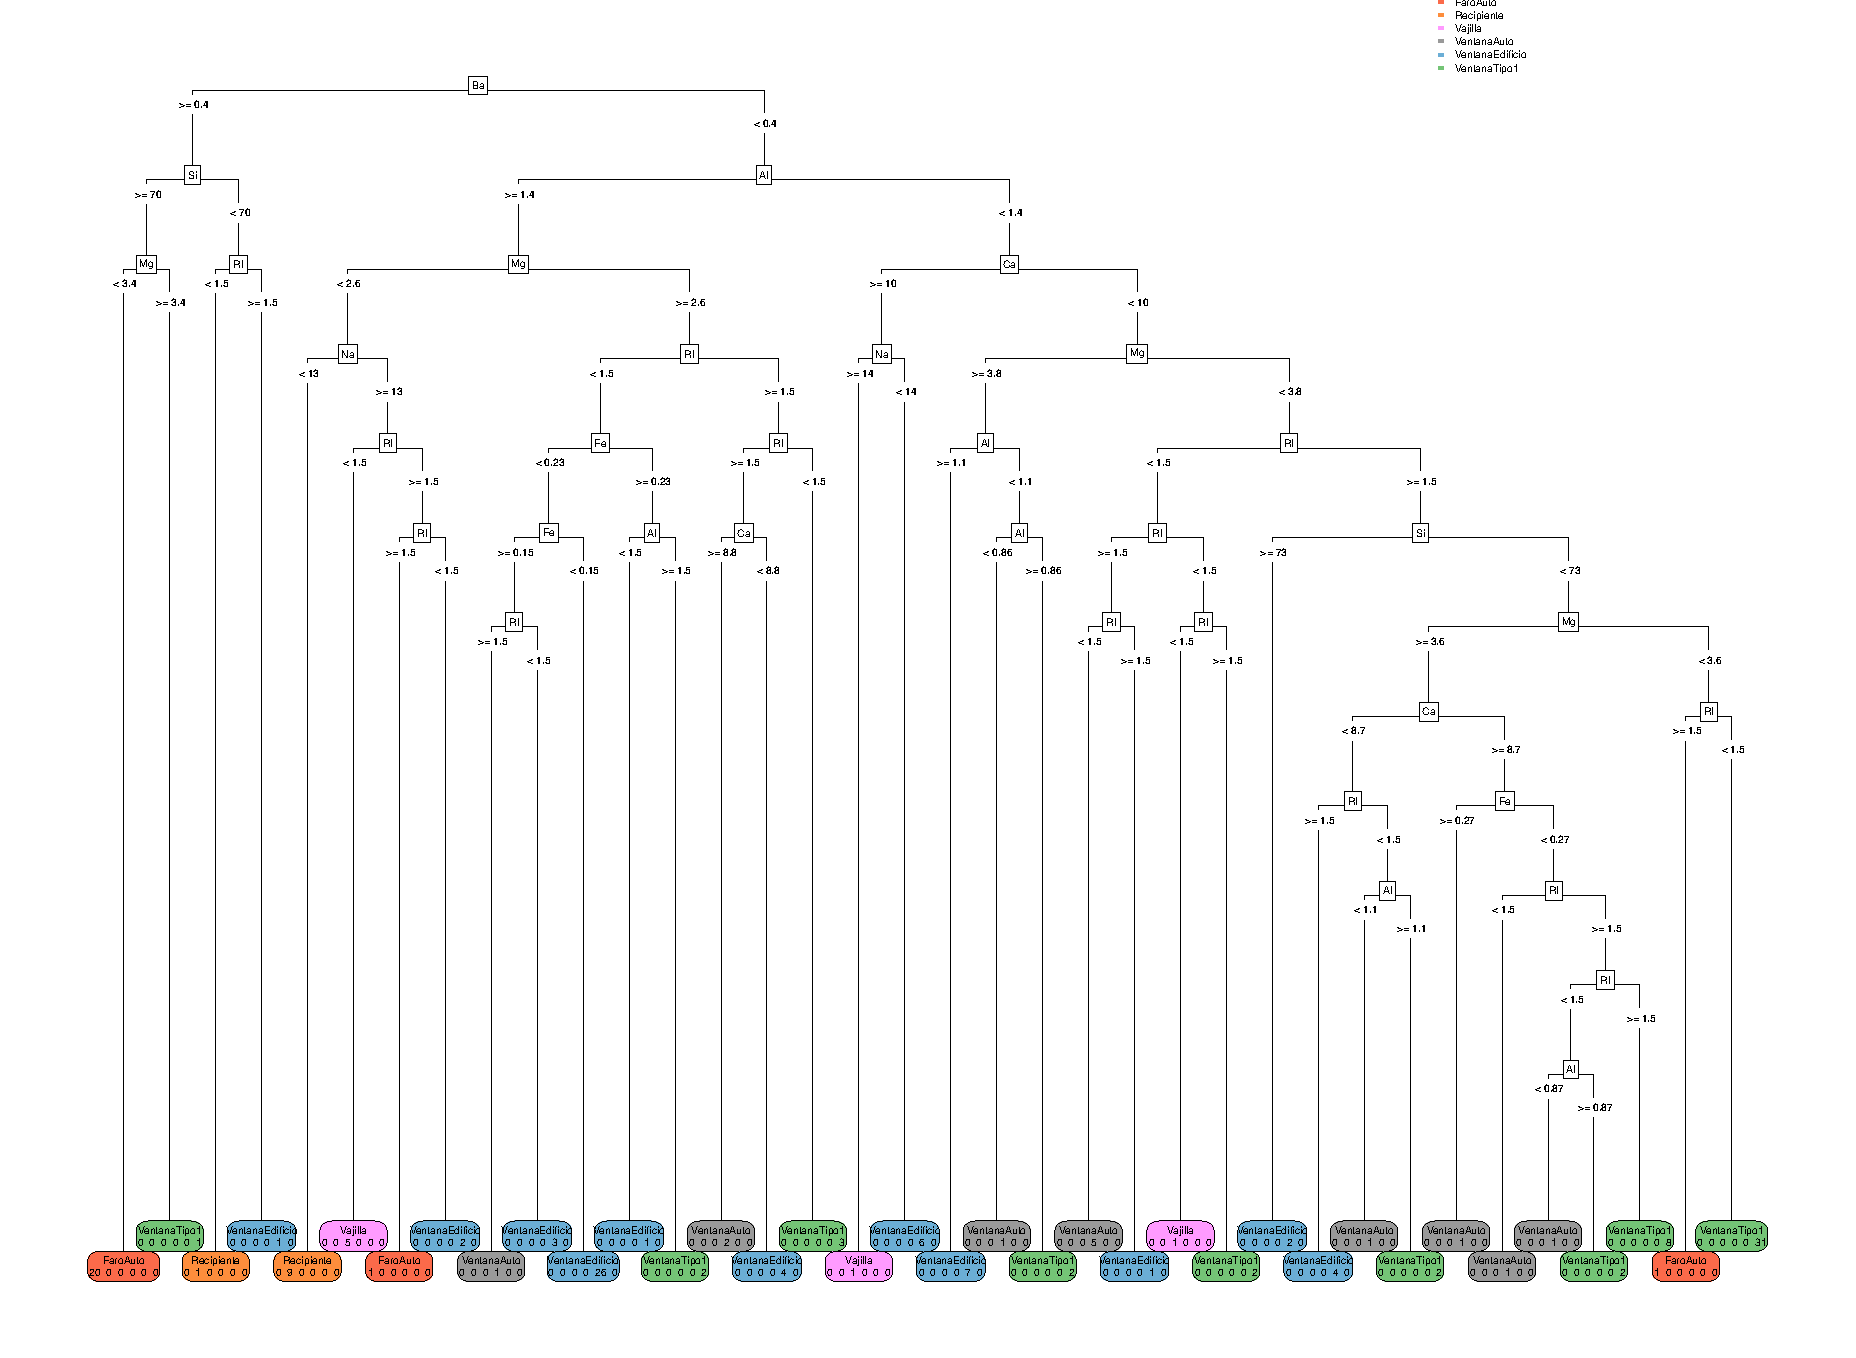
\includegraphics[width=\linewidth]{../Ejercicio-2/ImagenesEjercicio2/bigtree.pdf}
	\caption{Árbol de decisión grande}
	\label{fig:add1grande}
\end{figure}
Y se grafica el error de cada modelo (calculado por cross validation) en función del parámetro de complejidad (cp).
\begin{figure}[H]
	\centering
	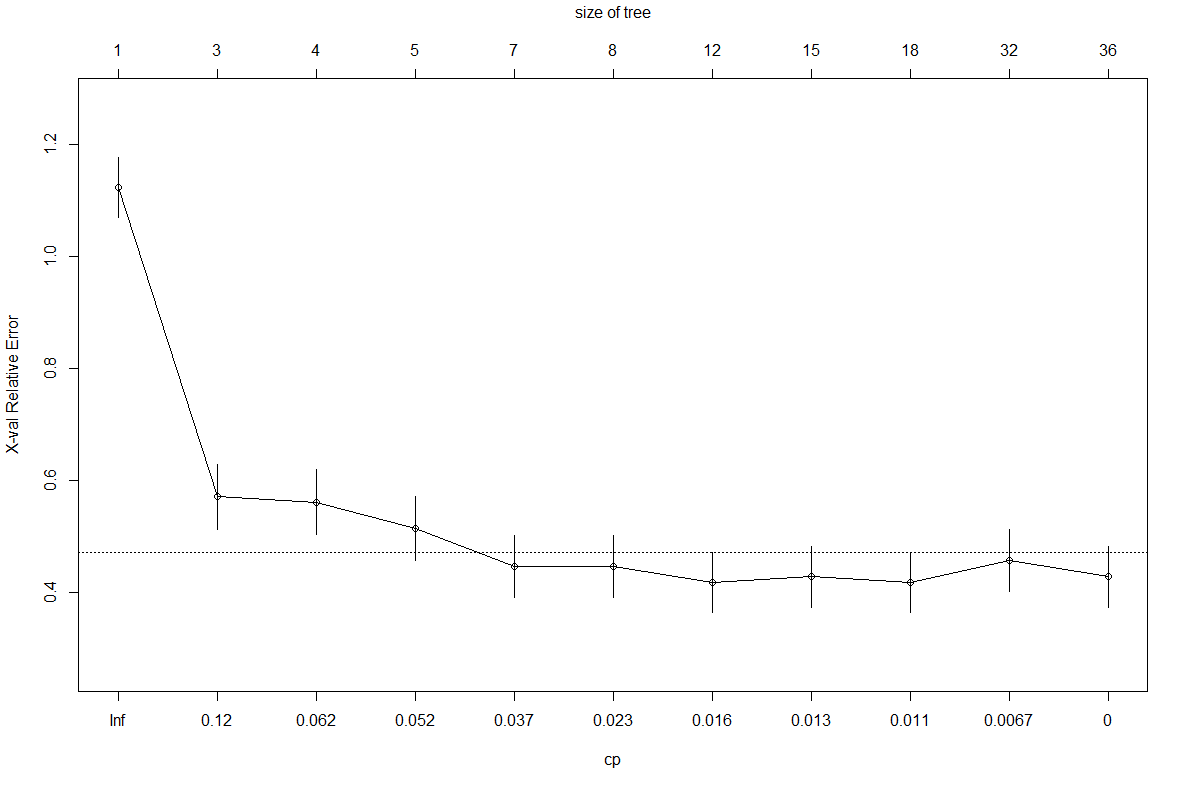
\includegraphics[width=\linewidth]{../Ejercicio-2/ImagenesEjercicio2/cp.png}
	\caption{Error en función del parámetro de complejidad}
	\label{fig:cpad}
\end{figure}
Se elije como cp aquel que con el menor número de hojas obtenga el menor error, 12 hojas, cp=0.016. A continuación se grafica el árbol de decisión final.
\begin{figure}[H]
	\centering
	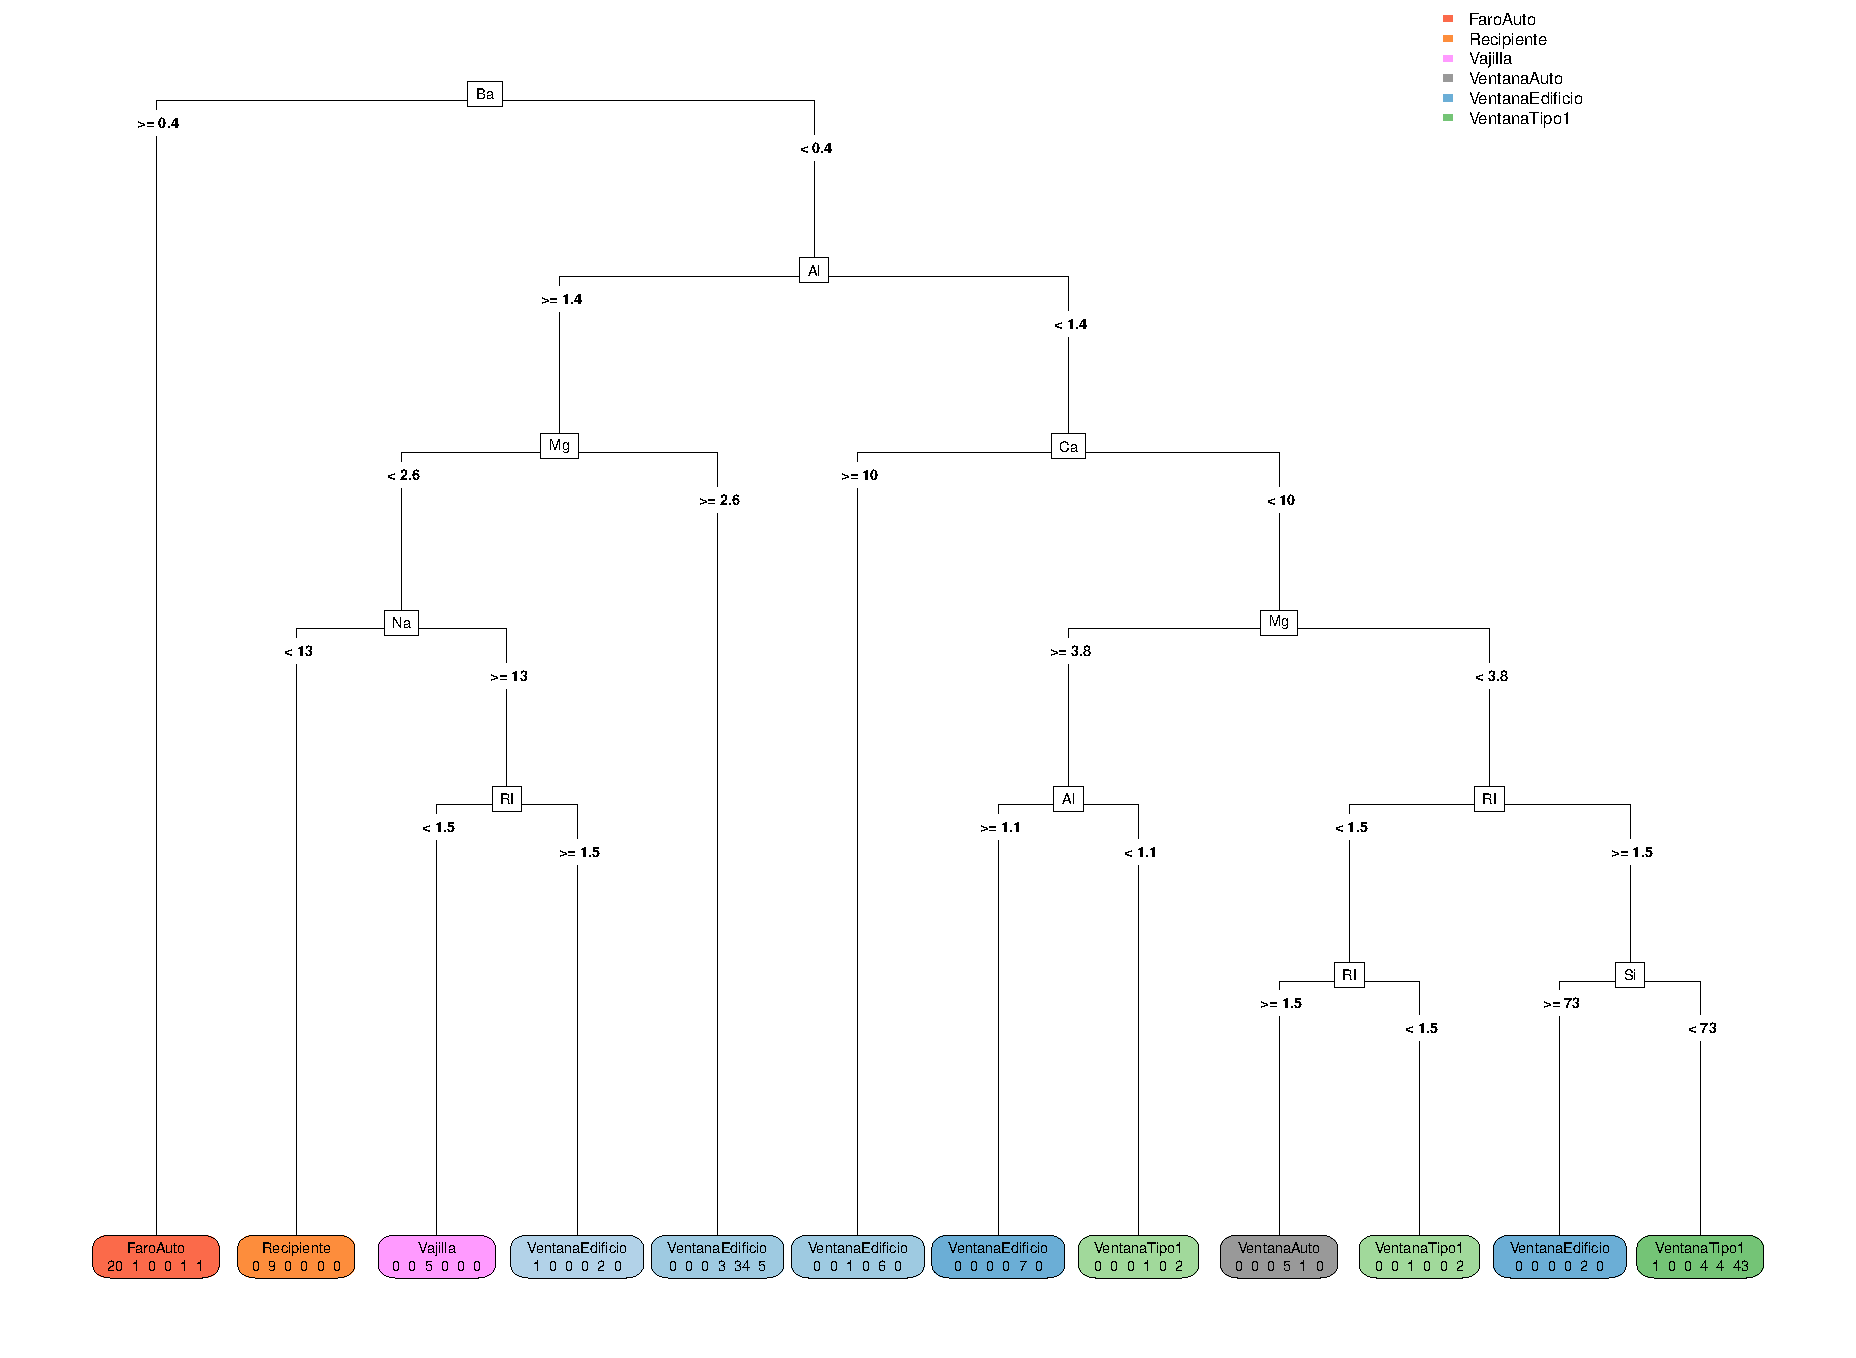
\includegraphics[width=\linewidth]{../Ejercicio-2/ImagenesEjercicio2/arbolpodado.pdf}
	\caption{Árbol de decisión podado}
	\label{fig:podado}
\end{figure}
Utilizando el metodo confusionMatrix se obtiene:

\begin{table}[H]
  \centering

    \begin{tabular}{l|ccccc}
    \multicolumn{1}{c}{} & \multicolumn{5}{c}{Reference} \\
    \cline{2-6}
    \multirow{6}[2]{*}{\rotatebox[origin=c]{90}{Prediction}} & FaroAuto & Recipiente & Vajilla & VentanaAuto & VentanaEdificio \\
    \cline{2-6}
          & 6     & 0     & 0     & 0     & 0 \\
          & 0     & 2     & 0     & 0     & 1 \\
          & 0     & 0     & 1     & 0     & 0 \\
          & 1     & 0     & 0     & 1     & 3 \\
          & 0     & 1     & 0     & 1     & 11 \\
          & 0     & 0     & 1     & 2     & 4 \\
    \end{tabular}%
      \caption{Matriz de confusión}
  \label{tab:confausion_matrix}%
\end{table}%

\begin{table}[H]
  \centering

    \begin{tabular}{ll}
    \hline
    \textbf{Accuracy} & 0.6923 \\
    \textbf{95\% CI} & (0.549, 0.8128) \\
    \textbf{No Information Rate} & 0.3654 \\
    \textbf{P-Value [Acc > NIR]} & 1.719e-06 \\
    \textbf{Kappa} & 0.5781 \\
    \textbf{Mcnemar's Test P-Value} & NA \\
    \hline
    \end{tabular}%
      \caption{Estadísticas generales}
  \label{tab:overall_staats}%
\end{table}%

\begin{table}[H]
  \centering

    \begin{tabular}{lcccccc}
    \hline
          & \textbf{Sensitivity} & \textbf{Specificity} & \textbf{Pos Pred Value} & \textbf{Neg Pred Value} & \textbf{Prevalence} & \textbf{Detection Rate} \\
    \hline
    \textbf{Class: FaroAuto} & 0.8571 & 1.0000 & 1.0000 & 0.9783 & 0.1346 & 0.1154 \\
    \textbf{Class: Recipiente} & 0.66667 & 0.97959 & 0.66667 & 0.97959 & 0.05769 & 0.03846 \\
    \textbf{Class: Vajilla} & 0.50000 & 1.00000 & 1.00000 & 0.98039 & 0.03846 & 0.01923 \\
    \textbf{Class: VentanaAuto} & 0.25000 & 0.91667 & 0.20000 & 0.93617 & 0.07692 & 0.01923 \\
    \textbf{Class: VentanaEdificio} & 0.5789 & 0.8788 & 0.7333 & 0.7838 & 0.3654 & 0.2115 \\
    \textbf{Class: VentanaTipo1} & 0.8824 & 0.8000 & 0.6818 & 0.9333 & 0.3269 & 0.2885 \\
    \hline
    \end{tabular}%
      \caption{Estadísticas por clase}
  \label{tab:class_astats}%
\end{table}%
Se puede ver como la accuracy aumento en un 5.77$\%$ y se puede notar como la sensibilidad para la vajilla aumento de 0 a 0.5, el aumento en sensibilidad para los dos tipos de ventanas de edificio, la variable specificity practicamente quedo igual, teniendo un aumento tanto para VentanaAuto como Recipiente.
\subsection{Parte Teórica}
En este trabajo se realizó un árbol de decisión, capaz de predecir que tipo de vidrio es una muestra, en base a su composición química. Para esto se realizo un análisis exploratorio de datos, para entender el dataset, ver que variables resultan relevantes y cuales no, al igual que un acondicionamiento de datos. Por otro lado se hicieron varios arboles de decisión, el primero es el que la librería rpart entrega por defecto dado el dataset. El segundo fue un árbol ampliado a su mayor longitud y el último es el optimizado en función del error de cada modelo. Finalmente se observaron las mejoras de del modelo optimizado versus el original.

\subsection{Código utilizado}
A continuación se muestra la totalidad del código utilizado.
\lstinputlisting[language=R]{../../../Code/Ej1b/Lambertucci.R}

%\end{document}
